\documentclass[tikz]{standalone}
\usepackage{amsmath}
\definecolor{bgcol}{HTML}{171D2B}
\definecolor{acc}{HTML}{F7B538}
\definecolor{barcol}{HTML}{3B82F6}
\begin{document}
\pagecolor{bgcol}
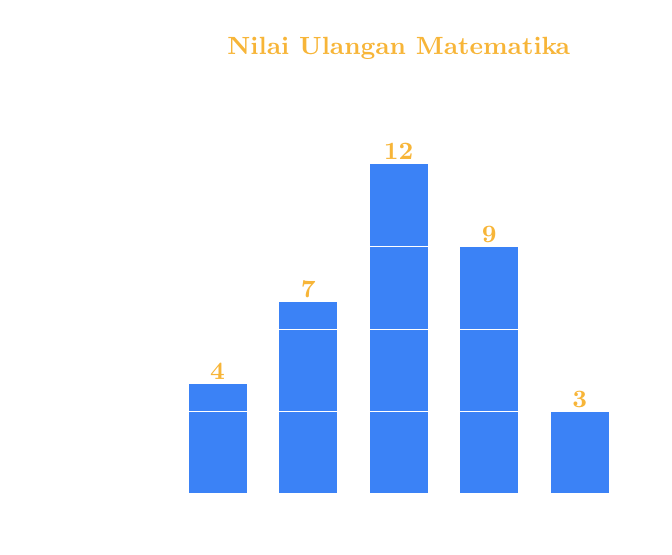
\begin{tikzpicture}[
  y=0.35cm, x=1.15cm,
  axis/.style={white, thick},
  label/.style={white, font=\small},
  value/.style={acc, font=\small\bfseries}
]
% frekuensi: 4, 7, 12, 9, 3  (interval 41-50 ... 81-90)
\foreach \x/\y/\lab in {0/4/{41--50}, 1/7/{51--60}, 2/12/{61--70}, 3/9/{71--80}, 4/3/{81--90}} {
  \fill[barcol] (\x-0.32,0) rectangle (\x+0.32,\y);
  \node[value] at (\x,\y+0.45) {\y};
  \node[label] at (\x,-0.55) {\lab};
}
\draw[axis] (-0.7,0) -- (4.7,0);
\draw[axis] (-0.7,0) -- (-0.7,15);
\foreach \y in {3,6,9,12,15} {
  \draw[white!40] (-0.7,\y) -- (4.7,\y);
  \node[label, anchor=east] at (-0.85,\y) {\y};
}
\node[label, rotate=90] at (-1.9, 7.5) {Frekuensi};
\node[label, acc, font=\small\bfseries] at (2, 16.2) {Nilai Ulangan Matematika};
\end{tikzpicture}
\end{document}
